\documentclass[10pt]{article}

\usepackage[a4paper,margin=1.75cm]{geometry}
\usepackage{amsmath,amssymb,booktabs,tabularx,array}
\usepackage{xcolor,tikz,fancyhdr}
\usepackage[hidelinks]{hyperref}
\usetikzlibrary{positioning,arrows.meta,calc}

\definecolor{ink}{HTML}{24324A}
\definecolor{blue}{HTML}{356A9A}
\definecolor{green}{HTML}{2F6B50}
\definecolor{rose}{HTML}{A84F70}
\definecolor{amber}{HTML}{A86512}
\definecolor{softblue}{HTML}{EAF2F8}
\definecolor{softgreen}{HTML}{EAF3ED}
\definecolor{softrose}{HTML}{F8E8EE}
\definecolor{softamber}{HTML}{FFF1D7}
\newcolumntype{Y}{>{\raggedright\arraybackslash}X}
\newcolumntype{P}[1]{>{\raggedright\arraybackslash}p{#1}}
\newcommand{\eid}[1]{\textcolor{green}{\texttt{#1}}}
\newcommand{\yes}{\textcolor{green}{\textbf{confirmed}}}
\setlength{\parindent}{0pt}
\setlength{\parskip}{5pt}

\pagestyle{fancy}
\fancyhf{}
\lhead{\textcolor{ink}{SPS Part 2: technical learning}}
\rhead{\textcolor{ink}{Goal-mode rerun, 16 July 2026}}
\cfoot{\thepage}
\setlength{\headheight}{14pt}

\begin{document}
\hypersetup{pageanchor=false}

\begin{titlepage}
\color{ink}
\vspace*{1.1cm}
{\Large\textbf{Part 2 technical learning report}\par}
\vspace{8mm}
{\huge\textbf{SPS: lineage, equations, and algorithm}\par}
\vspace{4mm}
{\Large Checked predecessors, correction, and claim limits\par}
\vspace{14mm}
\rule{\linewidth}{1.1pt}
\vspace{7mm}

{\large\textbf{Result in one sentence}\par}
\vspace{2mm}
SPS adapts the path-space sampler family to lattice field theory and uses
the full trajectory ratio as an extended-space independence-MH correction.

\vspace{8mm}
\begin{tabularx}{\linewidth}{@{}P{3.6cm}Y@{}}
\toprule
Question & Answer from the checked sources \\
\midrule
Did SPS introduce path-space sampling? & No. PIS and DDS already train
stochastic paths for unnormalized targets. \\
Did SPS first learn both directions? & No. CMCD already adapts coupled
forward and backward drifts. \\
What is different here? & Independent drift networks, learned scalar
diffusion, a lattice implementation, and extended-space trajectory IMH. \\
What is not established? & First-ever priority, isolated component benefit,
support robustness, or matched total-cost speedup. \\
\bottomrule
\end{tabularx}

\vfill
{\large Moxian Qian\par}
{\normalsize T0--T3 verified; T4--T5 not requested\par}
\vspace{2mm}
{\small Source IDs and paper anchors are retained in the companion Markdown
and CSV files.\par}
\end{titlepage}
\hypersetup{pageanchor=true}

\section{Question and reading contract}

The task was not to summarize SPS in isolation. It was to determine which
parts were already present in PIS, DDS, CMCD, and stochastic normalizing
flows, then reconstruct the corrected SPS algorithm without overstating
novelty. Five exact paper versions were read at C4 level and passed the
native R0--R6 record validator.

\begin{tabularx}{\linewidth}{@{}P{1.25cm}P{3.5cm}P{2.2cm}Y@{}}
\toprule
ID & Paper & Exact version & Role in the subtraction \\
\midrule
P002 & Path Integral Sampler & 2111.15141v2 & controlled path and trajectory weights \\
P003 & Denoising Diffusion Samplers & 2302.13834v2 & OU reverse path KL \\
P004 & Controlled Monte Carlo Diffusions & 2307.01050v12 & paired drift adaptation \\
P007 & Stochastic normalizing flows & 2201.08862v3 & lattice path ratios and reweighting \\
P001 & Stochastic Path Sampler & 2606.13790v1 & focal lattice sampler and trajectory IMH \\
\bottomrule
\end{tabularx}

P004 was added during reading because P001 states that CMCD already learns
forward and backward drifts. It is therefore required for the novelty check.

\section{Checked lineage}

\begin{center}
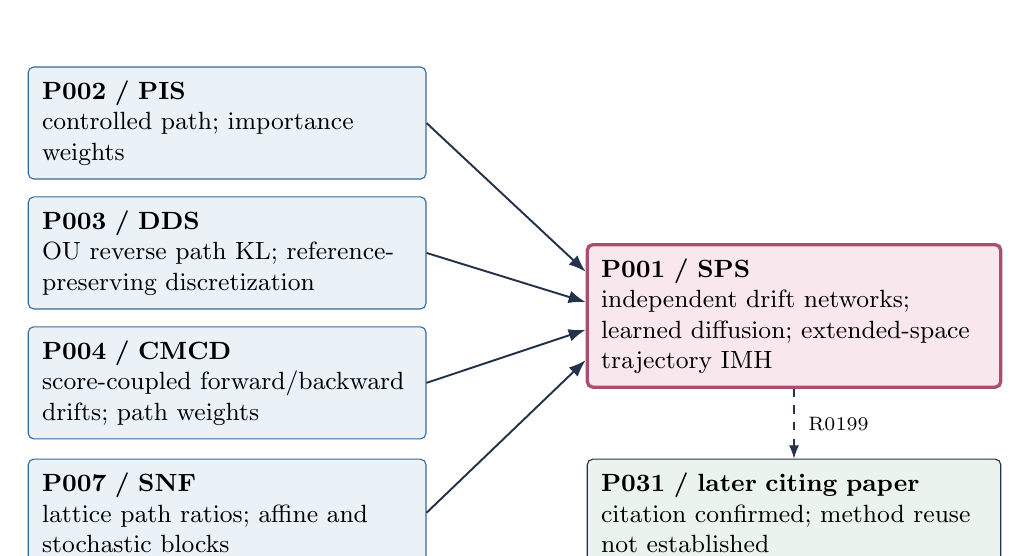
\begin{tikzpicture}[
  >=Latex,
  every node/.style={font=\small,align=left,rounded corners=2pt,inner sep=5pt},
  pred/.style={draw=blue,fill=softblue,text width=4.7cm},
  focal/.style={draw=rose,fill=softrose,line width=1.2pt,text width=4.9cm},
  later/.style={draw=ink,fill=softgreen,text width=4.9cm},
  edge/.style={->,draw=ink,line width=0.7pt}
]
\node[pred] (pis) at (0,0) {\textbf{P002 / PIS}\\controlled path; importance weights};
\node[pred] (dds) at (0,-1.65) {\textbf{P003 / DDS}\\OU reverse path KL; reference-preserving discretization};
\node[pred] (cmcd) at (0,-3.30) {\textbf{P004 / CMCD}\\score-coupled forward/backward drifts; path weights};
\node[pred] (snf) at (0,-4.95) {\textbf{P007 / SNF}\\lattice path ratios; affine and stochastic blocks};
\node[focal] (sps) at (7.2,-2.45) {\textbf{P001 / SPS}\\independent drift networks; learned diffusion; extended-space trajectory IMH};
\node[later] (later) at (7.2,-4.95) {\textbf{P031 / later citing paper}\\citation confirmed; method reuse not established};
\draw[edge] (pis.east) -- ([yshift=16pt]sps.west);
\draw[edge] (dds.east) -- ([yshift=5pt]sps.west);
\draw[edge] (cmcd.east) -- ([yshift=-5pt]sps.west);
\draw[edge] (snf.east) -- ([yshift=-16pt]sps.west);
\draw[->,dashed,draw=ink] (sps) -- node[right,font=\scriptsize] {R0199} (later);
\end{tikzpicture}
\end{center}

Direct-citation relations: P002/R0171, P003/R0177, P004/R0178, and
P007/R0172. R0199 confirms a later citation only. Dijkstra set the reading
order; paper sections and equations support the claims.

\section{Predecessor subtraction}

\small
\begin{tabularx}{\linewidth}{@{}P{2.25cm}P{3.15cm}Y P{2.6cm}@{}}
\toprule
Dimension & Already present & SPS form & Decision \\
\midrule
Path sampling & PIS and DDS learn paths for unnormalized targets
& Discrete lattice Langevin path & inherited family \\
Path objective & PIS, DDS, CMCD, and SNF use path costs or path ratios
& $D_{KL}(q_F\Vert\widetilde q_B)$ & formulation differs \\
Both directions & CMCD adapts score-coupled forward/backward drifts
& independent drift networks plus learned $\sigma_\theta(t)$
& difference confirmed; benefit open \\
Lattice path branch & SNF combines stochastic updates and learned affine maps
& learned stochastic drift kernels without invertible affine blocks
& architecture changed \\
Correction & predecessors use trajectory weights or reweighting
& full-trajectory extended-space IMH
& narrowest checked difference \\
Efficiency & papers report incompatible ESS, error, or correlation metrics
& SPS reports chain autocorrelation and wall times
& no speed ranking \\
\bottomrule
\end{tabularx}
\normalsize

The current sources support a design difference. They do not support a
\emph{first-ever} claim. Establishing priority would require a separate
high-recall search for earlier auxiliary-variable and path-space MH
constructions.

\section{How the corrected SPS algorithm works}

\begin{enumerate}
\item Draw $s_0\sim\pi_0$ from the tractable Gaussian prior.
\item Simulate a complete forward path with $K_{\theta,F}$ and
  $\sigma_\theta(t)$; retain every Gaussian transition factor.
\item Evaluate $K_{\theta,B}$ and the backward transition factors on the same
  path.
\item Train both drifts and the diffusion network by minimizing the sampled
  forward/unnormalized-backward path log-ratio.
\item Generate an independent new path and retain its path-dependent proposal
  ratio.
\item Compare the proposed and current extended paths with Eq.~(2.19);
  accept the proposed endpoint or retain the current one.
\item Measure observables and autocorrelation on the corrected endpoint chain.
\end{enumerate}

\begin{align}
s_{i+1}
 &=s_i+\sigma_\theta^2(t_i)K_{\theta,F}(s_i,t_i)\Delta t
   +\sigma_\theta(t_i)\xi_i\sqrt{\Delta t},
   &&\text{P001 Eq.~(2.2)},\\
D_{KL}
 &=\int dq_F(\tau)\log\frac{dq_F(\tau)}{d\widetilde q_B(\tau)},
   &&\text{P001 Eq.~(2.13)},\\
P_{\mathrm{acc}}
 &=\min\!\left[1,
\frac{\widetilde\pi(s_T')T(s_T'\!\to s_T)}
     {\widetilde\pi(s_T)T(s_T\!\to s_T')}\right],
   &&\text{P001 Eqs.~(2.18)--(2.19)}.
\end{align}

The first equation generates a path, the second trains its forward/backward
balance without knowing $Z$, and the third restores target invariance if the
proposal covers the target support. Evidence: \eid{E-260613790-M} and
\eid{E-260613790-L}.

\section{Correction mechanism}

\begin{tabularx}{\linewidth}{@{}P{1.2cm}P{3.0cm}Y P{3.25cm}@{}}
\toprule
Paper & Finite-training output & Trajectory information & Correction object \\
\midrule
PIS & weighted endpoints & $dQ^*/dQ^u$ & importance estimator \\
DDS & approximate endpoints plus $\widehat Z$ & $dP^{ref}/dQ_\theta$ & importance estimator \\
CMCD & approximate endpoints plus weight & forward/backward path ratio & importance estimator \\
SNF & weighted lattice paths & reverse/forward transition ratio & reweighted observable \\
SPS & correlated corrected chain & path-dependent proposal ratio & extended-space IMH \\
\bottomrule
\end{tabularx}

All five methods use full-path information but use it differently. This
comparison prevents an incorrect claim that SPS introduced trajectory
correction.

\section{Evidence and claim limits}

\small
\begin{tabularx}{\linewidth}{@{}P{2.3cm}Y P{3.7cm}@{}}
\toprule
Claim & Source-supported result & Boundary \\
\midrule
Corrected observables & SPS+IMH follows the reported HMC magnetization and
susceptibility across the tested 2D $L\times8$ scan
(\eid{E-260613790-R}) & benchmark-specific; uncorrected tails and multimodal
regions deviate \\
Acceptance & about 0.60--0.76 at $L=16$ and 0.45--0.62 at $L=64$
(P001 Fig.~6) & acceptance is not total efficiency \\
Timing & about 1.1--1.2 h training and 1.1--2.1 min generation across the
reported sizes (P001 Table~4) & no matched HMC GPU-hour ratio
(\eid{E-260613790-L}) \\
Autocorrelation & about 0.5 for SPS+IMH and about 160 for HMC at the reported
$L=64$, $\kappa=0.27$ point (P001 Fig.~8) & IMH steps and HMC trajectories are
different units; not a speed ratio \\
Exactness & extended-space IMH targets the physical distribution
(\eid{E-260613790-M}) & proposal support is required
(\eid{E-260613790-L}) \\
\bottomrule
\end{tabularx}
\normalsize

\textbf{Allowed:} In the tested two-dimensional benchmark, corrected SPS
reproduces the reported HMC observables; the paper leaves a matched
total-cost comparison open.

\textbf{Do not write:} SPS is universally 320 times faster than HMC.

\section{Validation and run accounting}

\begin{tabularx}{\linewidth}{@{}P{1.0cm}Y P{2.4cm}@{}}
\toprule
Level & Demonstration & Status \\
\midrule
T0 & exact identities, versions, URLs, pages, and hashes & \yes \\
T1 & bounded explanation of problem, mechanism, result, and limits & \yes \\
T2 & six aligned formula roles and five validated reading records & \yes \\
T3 & ordered training, proposal, extended-state correction, and output & \yes \\
T4 & equation-to-code symbol mapping & not requested \\
T5 & numerical reproduction & not requested \\
\bottomrule
\end{tabularx}

Goal-mode telemetry is recorded in \texttt{goal\_usage\_snapshots.csv}. The
counter is the Goal runtime's cumulative \texttt{tokensUsed}, not API billing
usage or monetary cost.

\begin{tabularx}{\linewidth}{@{}P{1.2cm}Y P{2.5cm}P{2.4cm}@{}}
\toprule
Stage & Work & Cumulative tokens & Cumulative seconds \\
\midrule
S00 & goal start & 0 & 0 \\
S01 & contract and Part 1 lock & 14,413 & 39 \\
S02 & exact source lock & 395,432 & 3,945 \\
S03 & five equation-level readings & 711,191 & 5,130 \\
S04 & predecessor subtraction and review & 763,038 & 5,396 \\
S05 & outputs and visual layout check & 915,839 & 5,817 \\
S06 & final pre-completion audit & 1,083,239 & 6,220 \\
S07 & Goal completion & 1,161,662 & 6,367 \\
\bottomrule
\end{tabularx}

\section{Companion audit files}

\begin{tabularx}{\linewidth}{@{}P{4.8cm}Y@{}}
\toprule
Artifact & What it records \\
\midrule
\texttt{paper\_reading\_record\_P*.md} & exact paper-level extraction and claim boundaries \\
\texttt{paper\_reading\_ledger.csv} & one-row comparison across the five core papers \\
\texttt{innovation\_delta.csv} & inherited, changed, inferred, and unresolved components \\
\texttt{equation\_code\_map.csv} & formula-to-algorithm trace; T4 fields explicitly not requested \\
\texttt{lineage\_learning\_path.mmd} & checked citation route and unresolved successor edge \\
\texttt{review\_core.md} & retained, weakened, rejected, and open claims \\
\texttt{goal\_usage\_snapshots.csv} & stage-by-stage Goal token and elapsed-time observations \\
\bottomrule
\end{tabularx}

\section{Source index}

\begin{itemize}
\item P001: \href{https://arxiv.org/abs/2606.13790}{arXiv:2606.13790v1},
  \eid{E-260613790-I}, \eid{E-260613790-M},
  \eid{E-260613790-R}, \eid{E-260613790-L}.
\item P002: \href{https://arxiv.org/abs/2111.15141}{arXiv:2111.15141v2},
  \eid{E-211115141-I}, \eid{E-211115141-M}, \eid{E-211115141-L}.
\item P003: \href{https://arxiv.org/abs/2302.13834}{arXiv:2302.13834v2},
  \eid{E-230213834-I}, \eid{E-230213834-M}, \eid{E-230213834-L}.
\item P004: \href{https://arxiv.org/abs/2307.01050}{arXiv:2307.01050v12},
  \eid{E-230701050-I}, \eid{E-230701050-M}, \eid{E-230701050-L}.
\item P007: \href{https://arxiv.org/abs/2201.08862}{arXiv:2201.08862v3},
  \eid{E-220108862-I}, \eid{E-220108862-M}, \eid{E-220108862-L}.
\end{itemize}

\end{document}
